\chapter{Literature Review} \label{chap:litreview}

\section{Introduction}
Hospitals often have limited funding, and therefore managing and utilising
their resources efficiently has always been a priority \cite{Walczak2003}.
One key measurement of hospital activity, health care utilisation, and hospital
cost is the patient length of stay \citep{Omachonu2004,Ng2006}. The length of
stay has been used in a wide variety of medical domains, such as burns
 \citep{Yang2010}, intensive
care \citep{Tu1993,Harper2005,Perez2006,Dybowski1996},
psychiatry \citep{Lowell1997}, and acute pancreatitis \citep{Pofahl1998}, in
order to assist hospitals in allocating beds and other patient management
resources as efficiently as possible. However, given the many different
conditions that hospitals manage, the length of stay of a patient is
not easy to predict \citep{Walczak2003}, especially upon a patient's admission.
Many methods have been explored in the literature, from the realm of statistics
to techniques in data mining, and they have been explored for many different
medical domains.

One of the more well-understood and widely used statistical methods for
predicting the length of stay is \textit{logistic regression} \citep{Tu1996}.
Logistic regression models are straightforward to construct and use via the
help of statistical software packages such as
SAS\footnote{SAS Institute, Cary, NC, USA}, and
also make the contribution of each independent variable to the final
prediction explicit. Thus they is easy to interpret when compared to more
``black box'' approaches such as artificial neural networks \citep{Adams2012}.
A wide variety of other statistical approaches have been proposed, notably:
various scoring systems from univariate analysis \citep{Adams2012,Lavoie2005},
linear regression \citep{Yang2010}, exponential models \citep{Clark2007},
survival analysis \citep{Vasilakis2005}, and Markov
models \citep{Perez2006,Jain1989,Kapadia2000}.

Out of the development of the various statistically-motivated models, data
mining techniques, particularly artificial neural networks,
began to become more widely adopted following a number of
early applications to length of stay prediction in intensive
care \citep{Tu1993,Dybowski1996}, in addition to disease diagnosis and mortality
prediction \citep{Silva2006}. Artificial neural networks are able to detect
complex and non-linear relationships between input and output variables and can
be developed using many different techniques. Much work has been done in using
neural networks to predict patient length of stay in various medical conditions
such as acute pancreatitis \citep{Walczak2003}, gastroenteritis \citep{Ng2006},
surgical intensive care \citep{Buchman1994,Tu1993} and
psychiatry \citep{Lowell1997}. Other data mining techniques have also been
applied, such as support vector machines and tree-based
methods \citep{Harper2005}.

Given the benefits to the hospital of accurate length of stay prediction,
this research aims to build upon improving length of stay prediction for trauma
patients by utilising state-of-the-art data mining techniques. Being able to
predict the length of stay for trauma patients is especially crucial because of
the scarcity of patient care resource in this area \citep{Yang2010}.
Additionally,
despite the wealth of research into length of stay prediction in various
medical domains, there has been little work done in generalising models from
one domain to another, or to predict a combination of outcomes (not only
length of stay, but mortality, or rehabilitation requirement). Being able to
do this would mean that hospital staff are better equipped to handle patient
cases and prepare for possible critical outcomes well in advance, resulting
in time and resources saved for both hospital and patient.

This literature review is structured as follows. We will first describe the
various statistical modelling techniques for predicting length of stay that
have been used in the literature, followed by a review of the data mining
techniques and how they compare in terms of accurately being able to predict
patient length of stay. The review will conclude with a summary and a
discussion on the gaps in the literature and how this work intends to address
those gaps.

\section{Statistical methods}
\subsection{Regression}
As we stated earlier, logistic regression is a commonly-used modelling
technique for prediction in the medical domain \citep{Tu1996}, and especially
in the trauma data analysis \citep{Gabbe2005}. A series of
predictor (independent) variables (or features) determine the probability of a
particular outcome by an equation of the form
\begin{equation}
\mathrm{log}\left(\frac{p}{1-p}\right) = \beta_0 + \beta_1X_1 + \beta_2X_2 + \dots + \beta_nX_n
\end{equation}
where $p$ is the probability of the desired outcome, $\beta_i$ are coefficients
associated with each variable, and $X_i$ are the values of the independent
variables \citep{Hosmer1989}. A stepwise selection algorithm is often used to
choose which variables to include in the model out of all available variables:
different algorithms produce different models which are then compared against
one another to find the best model. Usually, a standard maximum-likelihood
procedure is followed in order to obtain values for the $\beta_i$'s, and models
can be tested using measures such as the area under the receiver operating
characteristic (ROC) curve (AUC) and the Hosmer-Lemeshow statistic.

This is the method that Gabbe et al. used in their study to identify factors
that contributed to trauma patient length of stay and use these factors to
subsequently predict length of stay \citep{Gabbe2005}. The prediction problem
they proposed was essentially a binary classification problem, to which
logistic regression is well suited \citep{Tu1996}: will length of stay be
\textit{less than 5 days}, or \textit{equal to 5 days}? They used a
\textit{backward} stepwise selection algorithm, whereby all available variables
were initially included in the model and then progressively eliminated if their
likelihood ratio (LR) test $P$-value was $>0.15$. Features could only be
re-included if $P<0.05$. For length of stay
prediction, this left them with 9 features out of the 15 that they originally
included. To validate their model, they used a data set collected from an
independent source which had slightly different statistical characteristics for
the various features and outcomes. Their length of stay prediction model was
found to have 95\% sensitivity and 24\% specificity, with an area under the ROC
curve (AUC) of 0.62. This indicates that the model is not able to discriminate
length of stay cases of less than 5 days and equal to 5 days (i.e., the two
desired outcomes) very well, and only does
slightly better than simply random guessing (which has AUC 0.50).

In a similar study, Dinh et al. sought to predict whether or not trauma
patients could be predicted to stay in hospital \textit{less than 2 days} or
\textit{greater than 2 days} \citep{Dinh2013a}.
They also used a logistic regression model and
selected their features using a stepwise selection algorithm with the same
$P$-value threshold (0.05). Even though we cannot compare their result to that
of Gabbe et al. above because the models were tested on completely different
data sets, it is interesting to note that the model obtained by Dinh et al.
had an AUC of 0.83 after bootstrap cross-validation\footnote{A technique of
sampling a single data set with replacement: e.g. given a set of 100 records,
we can create a bootstrap sample that also contains 100 records which contains
records from the original set drawn at random with replacement. This means that
some records may appear in the bootstrap sample more than once and some may not
appear at all. In the work of Dinh et al., they performed this sampling 500
times (thereby creating 500 data sets) to evaluate the performance of their
model}. This indicates that the model had much better discrimination between
the two values for the outcome. Again, while we cannot directly compare, the
better performance could be due to the availability of more relevant features
to the outcome: Gabbe et al. included very few features specific to trauma
such as place of injury and mechanism of injury \citep{Gabbe2005} whereas Dinh
et al. also had variables for certain kinds of injuries (such as if it was
penetrating), specific body regions that were affected, and whether operations
were required. Given the nature of the length of stay, it would seem that Dinh
et al. derived a model that had included features with more explanatory power
on the outcome, thereby obtaining better results. This idea is consistent with
Buchman et al., who used logistic regression to predict the probability of a
patient in a surgical intensive care unit staying greater than a
week \citep{Buchman1994}.

While logistic regression is simple to use and its results straightforward
to interpret, the above approaches have described a coarse two-class prediction
problem, namely that of predicting the length of stay less than or greater than
a certain threshold. A number of \textit{linear} regression models have been
explored in the literature that examine the task of predicting length of stay
as a continuous quantity.

The key difference between linear and logistic regression is the nature of the
dependent variable: in linear regression it is treated as continuous (i.e., it
can take on any value), whereas in logistic regression it is a dichotomy of
only two values. The works discussed above only considered predicting the
length of stay as two possible outcomes, less than or greater than a particular
threshold of time. We have already stressed the importance of accurate length
of stay prediction for hospitals, and therefore it makes sense that attempting
to predict length of stay as a continous variable could give us more accurate
and useful insight and facilitate better resource allocation.

Yang et al. \citep{Yang2010} used a linear regression model as the baseline for
performance benchmarking when trying to predict the length of stay of burn
patients. Interestingly, unlike the logistic regression models discussed above,
they did not perform any feature selection when constructing their models and
found that this gave better performance against models constructed using
correlation-based feature selection\footnote{Abbreviated CFS, correlation-based
feature selection is a technique of choosing which independent variables to
include in a model based on the hypothesis that good variable subsets should
be highly correlated with the dependent variable but not with each
other \citep{Hall2000}.}. Unlike other studies into length of stay prediction,
they also looked at predicting the length of stay at various stages of the
clinical process, rather than simply at admission. By making predictions
at the admission, acute, and post-treatment stages, they were able to decrease
their predictions' mean absolute error (MAE) from 9.532 days at admission, to
6.314 days at post-treatment, where MAE is defined as
\begin{equation}
MAE = \frac{\sum_{i=1}^n |\mathrm{PredictedLOS}_i-\mathrm{ActualLOS}_i|}{n}
\end{equation}
and PredictedLOS$_i$ is the predicted length of stay for the $i$-th instance,
ActualLOS$_i$ is the actual length of stay for the $i$-th instance, and $n$
is the total number of instances. Their approach was very much appropriate to
their medical domain (burn patients) as they tended to have longer lengths of
stay (which is more suitable for linear regression rather than logistic
regression) and the extended period of stay means that there will be enough
data from several phases of the clinical process for such patients. It is
difficult to apply such a phase method to our problem of trauma length of
stay prediction, however, as there is no standard clinical process due to
the varying nature of trauma causes and the lengths of stay are typically not
as long.

\subsection{Markov models}
There have been a number of studies attempting to model the length of stay
using discrete-time Markov processes. Kapadia et al. constructed a transition
probability matrix using 4 states for a pediatric intensive care unit (ICU)
application \citep{Kapadia2000}:
\begin{center}
\begin{tabular}{l|llll}
& Low & Medium & High & Exit \\
\hline
Low & 0.309 & 0.223 & 0.024 & 0.444 \\
Medium & 0.137 & 0.513 & 0.096 & 0.254 \\
High & 0.086 & 0.364 & 0.379 & 0.171 \\
Exit & 0 & 0 & 0 & 1 \\
\end{tabular}
\end{center}
From the matrix, we can say that the probability of transitioning from state
`Medium' to state `Low' is 0.137. Note that each row sums to 1, and that `Exit'
is an absorbing state: once entered, one can only re-enter the `Exit' state
with 100\% certainty. This represents patients leaving the ICU. How did they
obtain these probabilities? From their data set, they classified each patient
with an appropriate state (Low, Medium, High) corresponding to the severity of
their illness based on a particular mortality score (PRISM), and did this daily
over a few months; this gave them patient records that were simply strings of
L, M and H. To calculate the probability of transitioning from `Medium' to
`Low', they counted all occurrences of `Medium' to `Low' transitions and
divided this by the number of all transitions out of `Medium', and repeated
this for every transition. Using the theory of Markov processes, they are able
to calculate the average time taken before a person enters the `Exit' state,
which is precisely the length of stay. They found that the Markov model fitted
the data well and produced predictions that were very close to the observed
results in the test set \citep{Kapadia2000}, indicating that using such models
justifies further investigation.

Perez et al. also used a Markov model to estimate the length of stay of
patients in a number of different destinations after one day of ICU admission
 \citep{Perez2006}. They created six models for different body regions and their
system had eight states. Using these models, they were able to obtain a
detailed breakdown prediction of how long each patient would be expected to
stay in a particular state given their injury. Their models had varying levels
of fit to the data, suggesting that some systems did not satisfy the Markov
property. Using such models gives practitioners a greater level of insight
into how patients are expected to progress through their particular situation
and allows them to prepare accordingly, rather than simply providing a number
for the length of stay. Clearly, there is an opportunity here to investigate
the types of medical problems that Markov modelling works well for, as well as
the problems that do not work so well.

\subsection{Other statistical techniques}
A number of other techniques have been used in length of stay prediction, which
we will describe briefly.
Yau et al. \citep{Yau2003} proposed a \textit{mixture regression model} in
modelling
length of stay to overcome the problem of correlated observations in hospital
data, which allowed them to predict neonatal length of stay across heterogenous
sub-groups (short-stay and long-stay). The idea is that these two sub-groups
have different length of stay patterns, and the length of stay of any patient
is just the probability of them being in one of these two groups (as well as
taking into account the underlying distribution of the group itself). Applying
this method to a set of neonatal length of stay data, they were able to
identify which input factors contributed to which component (short or long
stay) and derive useful insight for hospitals.

Clark et al. used a similar idea in their study of mortality and length of stay
prediction \citep{Clark2002}, by employing \textit{piecewise exponential models}
to model different probabilities of transition over distinct periods of time.
They obtained predictions for the length of stay and the probability of
survival that were fairly close to the actual outcome, for different age groups
and trauma types. These approaches have the advantage of being able to fit the
data more closely, but are more complex to estimate and use.

\section{Data mining methods}
Data mining is the analysis of (often large) observational data sets to find
unsuspected relationships and to summarise the data in novel ways that are both
understandable and useful to the data owner \citep{Hand2001}. Compared to
traditional statistical, it is a relatively recent field that emerged in the
1990s, and has
given researchers a variety of new tools to analyse and understand biomedical
datasets \citep{Bellazzi2008,Yoo2012}. Bellazzi \& Zupan \citep{Bellazzi2008}
have written a
comprehensive review paper of data mining techniques in clinical prediction
settings, and we refer the reader to their article for a more detailed
treatment of the techniques and their applications. Here we will describe the
major methods in the context of their application to predicting hospital length
of stay.

\subsection{Artificial neural networks}
Artificial neural networks have been widely used in clinical prediction
following their use in diagnosing acute myocardial infarction and various
applications in radiology \citep{Baxt1995}.
One of the earliest applications of neural networks to
length of stay prediction was by Tu \& Guerriere, who used a neural network
with the following structure \citep{Tu1993} to predict length of stay in
intensive care following cardiac surgery:
\begin{figure}[h]
\caption{}
\centering
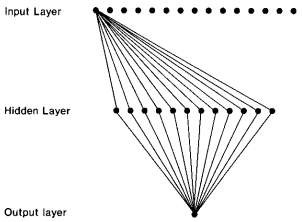
\includegraphics[scale=0.95]{images/a2-nn}
\end{figure}

There are 15 nodes (or ``neurons'') in the input layer, one for each of the
input features (predictor variables). For each example in the training set,
the input variable values are presented to the corresponding node in the input
layer, which are then propagated into the hidden layer and subsequently the
output layer. At the hidden layer, each of the 12 nodes sums the weighted
value of the 15 inputs (weighted value = input value $\times$ connection
weight), applies a non-linear activation function (usually the sigmoid function
$\frac{1}{1+e^{-t}}$), and sends this value as its output to the next layer
(in this case, the output layer). The single output node sums the 12 values
it receives from the nodes in the hidden layer and applies the same activation
function to produce a value between 0 and 1 that indicates the class.

The neural network is commonly ``trained'' by the backpropagation algorithm.
Once the network predicts a certain value for the given input record, this
predicted value is compared to the actual (or known) value, an error is
calculated and the connection weights are adjusted in order to minimise the
error quantity, which was the root mean square error in Tu \& Guerriere study.
The training is complete when the error has converged to a minimum value.

Using this technique,
Tu \& Guerriere wanted to predict whether a patient was going to stay
\textit{less than 2 days} or \textit{more than 2 days} following cardiac
surgery. After testing their trained neural network on the test data, they
found that it had an AUC of 0.6960, indicating a reasonable amount of
discriminating ability between the two outcomes. Even though we cannot compare
their result to any of the studies conducted on length of stay prediction
using logistic regression techniques, there are a number of well-known reasons
why neural networks are advantageous to modelling complex clinical situations:
\begin{enumerate}
\item Neural networks are able to model arbitrarily complex relations between
independent and dependent variables \citep{Tu1996,Buchman1994}, especially if
the relation is of a non-linear nature
\item Neural networks are able to handle models where the features (independent
variables) are not completely independent of each other
\item Neural networks can be ``trained'' in different ways, which changes their
predictive power -- this has been studied by Walczak et al. \citep{Walczak2003},
discussed in the next section
\end{enumerate}

However, there were a few difficulties in using the neural network as Tu \&
Guerriere discovered, which are problems often cited in the use of such
networks. These include a high sensitivity to the starting parameters (such as
network architecture\footnote{For example, how many hidden layers to have, and
how many nodes in each hidden layer. The difficulty of finding the right
architecture is pointed out by Tu \& Guerriere themselves -- in their paper
they state, ``The optimal structure of the neural network model was determined
by `trial and error' ''.}
and learning rate\footnote{A constant that is set by the
network developer that governs how much the connection weights should adjust at
each iteration of the training algorithm.}), as well as the difficulty in
inducing sensible rules from the model (even by domain
experts) \citep{Bellazzi2008}. Additionally, they are also prone to overfitting
and require substantially more computational power to train when compared to
the standard logistic regression technique, and do not always perform
better \citep{Harper2005}. A number of studies have attempted to address some of
these issues in length of stay prediction, building on from Tu \& Guerriere's
work, and these will be described in the next section.

\subsection{Extensions to the artificial neural network model}
Buchman et al. published a comparison of the performance of logistic regression
and neural networks on predicting whether or not patients would stay greater
than 7 days in a surgical intensive care unit \citep{Buchman1994}. Instead of
using one type of training algorithm as Tu \& Guerriere did, they obtained
results from three different neural network algorithms: backpropagation (the
standard against which other training methods are compared), probabilistic, and
generalised regression. Probabilistic neural networks are trained by a single
pass over the training data and use Bayes strategies and Parzen windows to
estimate a probability density function for prediction. Generalised regression
neural networks allow the definition of arbitrarily complex regression surfaces
which allows for greater modelling power and is able to produce continuous
values instead of simply a binary classification \citep{Sprecht1991}. They found
that all three neural networks performed noticeably better than the logistic
regression model, but that they all achieved fairly similar results (by the ROC
test). However, the AUC for the four models were not given.

Dybowski et al. decided to address the problem of neural network architecture
by applying a genetic algorithm approach to selecting the best
structure \citep{Dybowski1996} --
an improvement from the ``trial and error'' method Tu \& Guerriere used. It is
interesting to briefly discuss their method even though they were interested
in predicting the outcome of critically ill patients in intensive care, rather
than the length of stay which is the focus of our work. The genetic algorithm
in choosing an optimal neural network structure is as
follows \citep{Dybowski1996}:
\begin{enumerate}
\item A large population of random neural networks is created, each with
a random number of nodes in three hidden layers.
\item Each neural network optimises
its connection weights with respect to the same data set using
backpropagation.
\item Each neural network is expressed as a string which represents the
substructure of the network -- this is the ``chromosome''.
\item The ``chromosomes'' are copied to form a new population whereby the
expected relative frequency of a chromosome is proportional to how well
its neural network performed -- this is the ``survival of the fittest''
aspect.
\item The replica chromosomes undergo crossover so that better-performing
components can be combined. Mutations are also present, through the random
modification of a chromosome.
\item The process is repeated until a best-performing neural network forms.
\end{enumerate}
Through this Dybowski et al. were able to show that successive ``generations''
of neural networks had greater AUC measures, indicating better predictive
ability. Additionally, after seven generations, they obtained a neural network
that had an AUC of 0.863 compared to 0.753 for an equivalent logistic
regression model.

Walczak et al. also attempted to address the problem of arbitrary neural
network structure in their study to predict length of stay in two hospital
settings, acute pancreatitis and pediatric trauma \citep{Walczak2003}. Instead
of a genetic algorithm approach, they generated and tested every possible
neural network with one or two hidden layers, the quantity of nodes in each
layer varying from $2N$ to $5N$ where $N$ is the number of nodes in the
preceding layer, with a step size of 5. To address overfitting they also
discarded any networks generated this way whose performance dropped after
an initial increase. This comprehensive approach gave them over 100
backpropagation neural networks to evaluate for each of the two medical
domains. 
Rowan et al. followed a similar
approach to mitigate the effect of neural network structure, but instead of
selecting a single optimal network, they used ensembles of neural networks
to improve predictive power \citep{Rowan2007}. Many different combinations of
trained neural networks were tested in order to find the combination with the
greatest classification power according to the AUC measure.

Additionally, Walczak et al. also examined not only backpropagation, which
is the training algorithm used by most of the applications, but also radial
basis function and fuzzy ARTMAP. Using the mean absolute difference, they
found that a single hidden layer backpropagation neural network performed
better than all other networks in pediatric trauma, and was able to predict
the length of stay to within 1 day for 52\% of all cases. They also obtained
promising results using the fuzzy ARTMAP method, which warrants further
investigation as this training method has not been applied to modelling
length of stay in other medical domains.

One concern that has been raised with the use of neural networks in prediction
is that they are usually trained once and are not subsequently re-trained with
new data to fine-tune their connections. This has been worked on by Lowell et
al. in predicting psychiatric length of stay \citep{Lowell1997}, and also by
Ng et al. who proposed an incremental learning approach for neural networks
and applied it to gastroenteritis length of stay data \citep{Ng2006}. Lowell et
al. trained an initial model in an earlier paper to predict the length of stay
of psychiatric patients, and then subsequently deployed this model to three
separate sites. Using the additional site-specific data to re-train the initial
neural network resulted in increased prediction accuracy of 3-15\% with a less
than 10\% change in the training data \citep{Lowell1997}. Ng et al. took a more
theoretical approach and proposed a mixture of experts neural network with an
incremental learning algorithm based on expectation-maximisation. They wanted
to investigate how the neural network trained all at once (batch-mode)
would perform against the same network trained all at once and then
incrementally with new records as they were obtained. This allowed for an
on-line prediction system which takes into account new data, which had not
been investigated very much in the area of length of stay prediction. They
applied their proposed technique to a set of gastroenteritis data, and found
that the incremental learning method had a lower mean absolute difference (MAD)
on the test set (indicating that predictions were generally closer to the
actual value), and had a greater proportion of predictions with MAD less than
or equal to 1 day (meaning that more of the incremental learning neural
network's predictions were accurate to within a day), compared to the standard
batch-mode learning method \citep{Ng2006}.

\subsection{Other data mining techniques}
As discussed, artificial neural networks have been used extensively in
predicting patient length of stay. However, a few other data mining techniques
have also been investigated, namely tree-based methods and support vector
machines.

In a review published in 2005, Harper compared the performance of four
classification algorithms on four different medical data sets, trying to
model five different scenarios \citep{Harper2005}. Two of these outcomes were
relevant to our work: one was predicting the length of stay in the intensive
care unit, and another was predicting the length of stay in a particular
hospital ward. The classification techniques he used were discriminant
analysis, regression, CART (classification and regression trees),
and artificial neural networks.

CART has been extensively used in medical decision making, and at its heart
involves an algorithm that is used to split the data set into sub-groups of
increasing similarity. At each node in the tree, the algorithm examines the
independent variables and splits the data set on the variable that produces
a node with the smallest variance (i.e., the greatest similarity). This is
continued until defined stopping rules are met. One of the major reasons that
such tree-based methods are more popular than neural networks in the
healthcare domain is that the rules it ``learns'' are very simple to extract
from the resulting tree, unlike the ``black box'' that neural networks commonly
are. Harper found that CART performed almost as well as neural networks in
predicting intensive care length of stay, and much better in predicting
hospital length of stay in terms of predicting accuracy (the only evaluation
statistic reported). He also found that CART was superior to regression, a
finding that Yang et al. also reported when predicting the length of stay of
burn patients \citep{Yang2010}.

Yang et al. investigated the performance of linear regression, M5 (another
tree-based classification method), and support vector machines in predicting
length of stay for burn patients. The difference between their tree method,
M5, with that of Harper (CART), is that the nodes contain linear regression
functions instead of the usual discrete (two-class) outputs that are used to
successively split the data set. Additionally, they also use support vector
machines (SVMs), perhaps the most powerful classification algorithm in terms of
predictive accuracy \citep{Bellazzi2008}. SVMs work on the principle that when
the data is represented in a high enough dimensional space, a linear hyperplane
can be found where the margin between two different records is as large as
possible. In figure \ref{svm} from Yoo et al. \citep{Yoo2012}, hyperplane 2
is the better plane because its margin is as large as possible. 
\begin{figure}[h]
\label{svm}
\caption{}
\centering
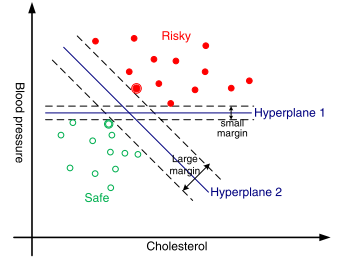
\includegraphics[scale=1.05]{images/a2-svm}
\end{figure}

However, because SVMs are typically
used for binary classification, Yang et al. adopted the technique of SVM
regression in order to predict a continuous value for the length of stay. The
idea is that the desired function would have the same margin-maximising
properties of the SVM, while being able to approximate the mapping between the
input domain and the real numbers \citep{Yang2010}. Evaluating the performance
of linear regression, M5 and SVM regression using the mean absolute error
(MAE) described earlier, they found that predictions from SVM regression
produced consistently lower MAEs across all three clinical stages when compared
to both the regression and tree-based methods. Regression was the poorest
performing predictor, which is consistent with many of the findings we have
discussed. The paucity of studies using tree-based methods and SVM techniques
to predict length of stay warrants more investigation, especially since the
SVM has high predictive power which would be useful to medical professionals.

It is important to note that length of stay prediction is most often a
\textit{supervised} problem, i.e. the desired outcome is known in the training
data, and we train our model to be able to produce the correct output based on
this data. Once we present this trained model with data with which the outcome
is not known, we expect that it will give us a reasonable prediction. This is
what all of the techniques described above fall under, and this is expected
given the nature of the problem. However, we should note that Huang et al. 
used an unsupervised technique, $K$-nearest neighbour clustering (KNN), in 
predicting the length of stay for clinical
treatment processes \citep{Huang2013}. Their approach assumes that similar
patients have a similar length of
stay. They define a patient trace to be a sequence of clinical events that are
performed on a patient, and define a similarity measure that follows the
principle of temporal edit distance\footnote{The \textit{edit distance}
between two states (or traces in this case) is the total ``cost'' of edit
operations (insertions, deletions, substitutions) required to change from
one state to another. The costs of each operation are defined based on the
application.}. Using this similarity measure, they find the $K$ most similar
patient traces to a given trace of unknown length of stay,
and find a similarity-weighted average of the lengths of stay
of the $K$ traces to produce a prediction for the unknown trace. They point
out some difficulty in determining the most suitable number for $K$, as well
as in measuring the performance of the algorithms due to the temporal nature
of the patient traces (very different error amounts depending on at which
time points measurements are taken at), but generally found that their
approach performed better than the widely used techniques of regression and
neural networks. This is a novel approach and should be investigated in further
studies for length of stay prediction.

\section{Conclusion}
Despite the wide range of statistical and data mining techniques that have been
used to predict the hospital length of stay, we have raised a few avenues for
further work throughout the literature review. Firstly, there has been no work
done to predict the length of stay of trauma patients using data mining
techniques, which is something worth investigating as trauma is a complex
medical condition. We have pointed out that there is also value in
investigating a number of the best data mining techniques, i.e. using more
than just neural networks. There is also value in investigating the performance
of such a model on data sets from different locations, since most studies are
only validated on one or two data sets. Additionally, length of stay prediction
has largely been restricted to specific medical domains, and therefore it is
worthwhile to examine if there are factors present in other domains which allow
for a more general model of the length of stay. 

